\documentclass[12pt]{article}

\usepackage[a4paper,  top=1.3in, bottom=1.4in, left=1.4in, right=1.5in]{geometry}

\usepackage[utf8]{inputenc}
\usepackage[T1]{fontenc}
\usepackage{amsmath}
\usepackage{amsfonts}
\usepackage{amssymb}


\usepackage{graphicx, float}
\usepackage{adjustbox}
\graphicspath{{images/}}

% \renewcommand{\figurename}{Slika}



\renewcommand{\baselinestretch}{1.2} % Line spacing

% Parskip and parindent
\setlength{\parindent}{0pt} % Begin of paragraph indentation
\setlength{\parskip}{1em} % Paragraph spacing

%--- for references ---------
\usepackage[
    backend=biber,
    style=numeric,
    sorting=none
    ]{biblatex}

\addbibresource{bibliography.bib}
\AtBeginBibliography{\vspace*{10pt}}
%----------------------------

%----------- toc ------------------------
\usepackage{tocloft}
\usepackage{fancyhdr}
% \setlength{\cftbeforesecskip}{0pt} % Adjust the spacing before section entries
% \setlength{\cftbeforesubsecskip}{0pt} % Adjust the spacing before subsection entries
%----------------------------------------

\begin{document}
\pagenumbering{gobble}  % Suppress page numbers initially

% Title Page
\newgeometry{top=1in, bottom=1in, left=1in, right=1in} % New margins for title page
\begin{titlepage}
    \begin{center}
        
        % add your university logo here
        % negative value moves the logo up
        \vspace*{-1in}
        
\includegraphics[width=0.4\textwidth]{raf_logo.png}

        % set font size to 14pt
        \vspace{1in}
        \Large
        \textbf{Review on the topic of}
        
        % set horizontal margin for the title to 1.5in and center it
        \vspace{1in}
        \Huge
        \textbf{Simultaneous localization and mapping (SLAM)}
        
        \vspace{1in}


            \fontsize{17pt}{17pt}\selectfont
            \textbf{Course: Robotics} \\
            \vspace*{1.5in}
            
            \begin{center}
            \normalsize
            \begin{tabular}{p{0.75\textwidth} p{0.5\textwidth}}
                \fontsize{14pt}{18pt}\selectfont   
                \textbf{Advisor:} & 
            
                \fontsize{14pt}{18pt}\selectfont
                \textbf{Student:} \\
                prof. Miloš Jovanović & Vanja Kovinić \\
            \end{tabular}
            \end{center}

            \vspace*{\fill}

            \normalsize
            Belgrade, 2025.


            
        \end{center}
    \end{titlepage}
    \restoregeometry % Restore original margins

    \newpage
    \newgeometry{top=1.3in, bottom=2.2in, left=1.4in, right=1.4in} % New margins for title page

    \tableofcontents

    \newpage
    \clearpage             % Move to a new page
    \pagenumbering{arabic} % Start using Arabic numerals
    \setcounter{page}{1}   % Set the counter to 1
    \section{Introduction to SLAM}
    \subsection{Definition and Problem Statement}
    \textbf{Simultaneous Localization and Mapping (SLAM)} represents one of the fundamental challenges in robotics. At its core, SLAM addresses a deceptively simple question: 
    \\ \textit{How can a mobile robot build a map of an unknown environment while simultaneously determining its own position within that map?} 
    \\ This seemingly straightforward task embodies a classic \textit{"chicken-and-egg"} problem - to create an accurate map, the robot needs to know its precise location,
    but to determine its location, it needs an accurate map.
    \\ The SLAM problem can be formally defined as the process of constructing or updating a map of an unknown environment while keeping track of an agent's location within it. 
    Mathematically, SLAM estimates both the trajectory of the robot ($X_{1} = {x_1, x_2, \ldots, x_t}$) and the map of the environment ($M$) given the observations ($Z_{1}$) and control inputs ($U_{1}$):
    \[p(X_{1}, M \mid Z_{1}, U_{1})\]
    This joint probability distribution encapsulates the inherent uncertainty in both the robot's position and the environmental map, recognizing that both must be estimated simultaneously.

    \newpage

    The technical challenges of SLAM extend beyond this core problem. Real-world implementations must contend with:
    \begin{enumerate}
        \item \textbf{Sensor limitations}: All sensors provide imperfect measurements with noise, limited range, and potential occlusions.
        \item \textbf{Data association}: Determining whether sensor observations correspond to previously observed landmarks or represent new features.
        \item \textbf{Loop closure}: Recognizing when the robot has returned to a previously visited location, allowing for correction of accumulated errors.
        \item \textbf{Computational efficiency}: Balancing accuracy with real-time performance requirements, especially on platforms with limited computing resources.
        \item \textbf{Environmental dynamics}: Managing changes in the environment, such as moving objects or changing conditions.
    \end{enumerate}

    \begin{figure}[h!]
        \centering
        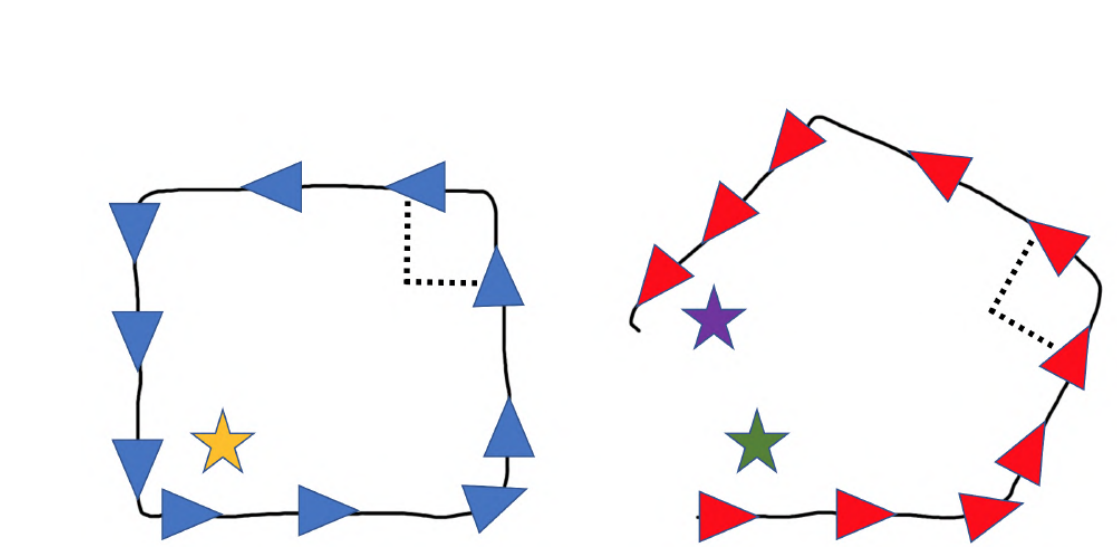
\includegraphics[width=0.8\textwidth]{loop_closure.png}
        \caption{The diagram shows loop closure in robot mapping. When a feature is recognized again (left), a constraint is added to correct the robot's trajectory. 
        If the feature is not recognized (right), errors in the estimated path remain uncorrected. \cite{loop_closure_img}}
        \label{fig:loop_closure}
    \end{figure}

    A successful SLAM system must integrate sensor data over time while accounting for uncertainties and constraints to produce a consistent representation of both the robot's path 
    and the surrounding environment.

    \newpage

    \subsection{Historical Context and Importance in Robotics}
    The development of SLAM techniques represents a crucial milestone in the evolution of autonomous robotics. Before SLAM, robots relied on pre-built maps or simple reactive behaviors, 
    severely limiting their autonomy and usefulness in unknown environments.
    The conceptual foundations of SLAM emerged in the 1980s through seminal work by researchers such as Hugh Durrant-Whyte and John J. Leonard \cite{seminal_paper}, who recognized 
    to the statistical correlations between landmarks in a map. However, the term "SLAM" itself was not coined until the early 1990s.

    The historical progression of SLAM research can be divided into several key phases:

    \begin{enumerate}
        \item \textbf{Early probabilistic approaches (1990s)}: The initial formulation of SLAM using Extended Kalman Filters (EKF) provided the mathematical framework for 
        handling uncertainty in both robot motion and sensing \cite{early_probabilistic_approaches}. These approaches were limited by computational complexity that scaled quadratically with the number of landmarks.
        \item \textbf{Particle filter methods (early 2000s)}: FastSLAM \cite{fast_slam} and other particle filter approaches offered improved performance for nonlinear systems and 
        non-Gaussian noise, enabling more robust implementations.
        \item \textbf{Graph-based optimization (mid-2000s)}: The formulation of SLAM as a sparse graph optimization problem led to more efficient solutions 
        that could handle larger environments and longer trajectories.
        \item \textbf{Visual SLAM systems (2007-2015)}: The incorporation of camera data enabled systems like MonoSLAM \cite{monoslam}, PTAM, and ORB-SLAM \cite{orb_slam}, which could operate 
        using only visual information without specialized ranging sensors.
        \newpage
        \item \textbf{Learning-based approaches (2015-present)}: The integration of deep learning methods has pushed the boundaries of SLAM performance, particularly 
        in feature extraction, depth estimation, and semantic understanding.
    \end{enumerate}

    The introduction of SLAM algorithms effectively gave robots a spatial intelligence - the ability to interpret, map, and navigate previously unseen environments without human guidance.
    Some of the most notable applications of SLAM include:
    \begin{itemize}
        \item \textbf{Autonomous vehicles}: Tesla's FSD system and Waymo's autonomous taxis implement sophisticated SLAM variants that fuse visual data with other sensor modalities. 
        Their ability to navigate complex urban environments relies not just on GPS (which fails in tunnels or urban canyons) but on real-time environmental mapping at centimeter-level precision.
        \item \textbf{Disaster response}: After the Fukushima nuclear disaster, robots equipped with RGBD-SLAM systems entered radiation-contaminated zones inaccessible to humans,
        creating 3D maps that enabled remote assessment of structural damage without endangering human lives \cite{fukushima_disaster}.
        \item \textbf{Domestic robotics}: The evolution of cleaning robots from random bouncers like early Roombas to the systematic path-planners seen in Roborock S7 models 
        illustrates how SLAM transformed consumer robotics from novelties into genuinely useful tools that can efficiently cover complex home layouts.
        \item \textbf{Mixed reality}: Apple's ARKit and Microsoft's HoloLens use visual-inertial SLAM to maintain stable positioning of virtual objects in the physical world, enabling 
        applications from surgical training to architectural visualization that rely on precise spatial registration.
    \end{itemize}

    \begin{figure}[h!]
        \centering
        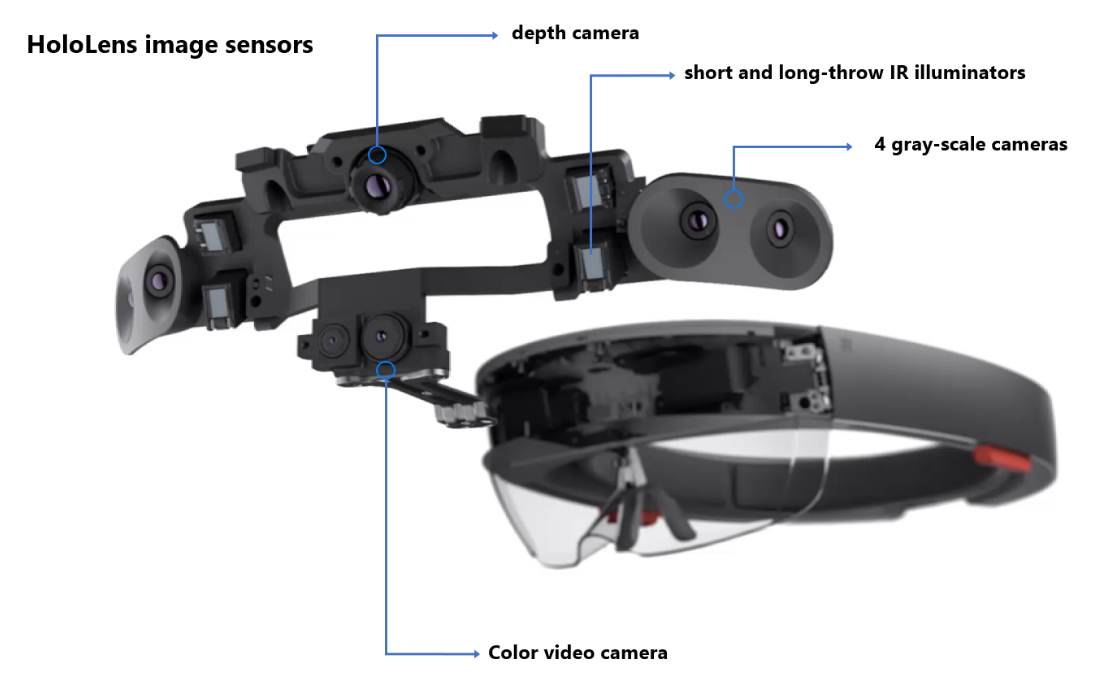
\includegraphics[width=0.7\textwidth]{mcsft_hololens.png}
        \caption{Microsoft HoloLens uses SLAM by fusing data from cameras, depth sensors, and IMUs to simultaneously track the headset’s position and map the environment. 
        This enables accurate placement of virtual objects in the real world for stable and immersive augmented reality experiences.}
        \label{fig:mcsft_hololens}
    \end{figure}


    \section{Fundamental Challenges in SLAM}

    \subsection{The Chicken-and-Egg Problem}
    
    The core paradox of SLAM is deceptively simple: to build an accurate map, a robot needs to know its precise location, but to determine its location accurately, it needs a reliable map. 
    This interdependence creates the \textit{"chicken-and-egg problem"} of SLAM.
    
    Consider a robot entering an unknown room. To map the room accurately, it must know exactly how far it has moved since entering. However, small errors in wheel encoders, IMU drift, or visual
    tracking cause position uncertainty to grow. 
    
    Without external references, these errors accumulate - a phenomenon known as "dead reckoning drift". After moving just a few meters, the robot's position estimate might be off by several centimeters, 
    causing all mapped features to be misplaced.
    This circular dependency manifests in two critical ways:
    
    First, position estimation errors directly propagate into the map. Imagine a robot that turns a corner and incorrectly estimates its rotation by 2 degrees. This small angular error will cause all subsequent 
    wall measurements to be tilted, creating a distorted map. When the robot later tries to localize using this faulty map, its position estimates become increasingly unreliable.

    Second, without correction mechanisms, uncertainty grows unbounded over time. A robot navigating a long corridor might start with centimeter-level position accuracy, but after traveling 20 meters, drift might increase 
    to decimeter-level errors. This uncertainty expansion makes long-term SLAM inherently unstable without additional constraints.
    
    The probabilistic SLAM framework addresses this by maintaining a joint distribution over both the robot's trajectory and map features:
    \[p(x_t, m | z_{1}, u_{1}, x_0)\]

    Where $x_t$ is the robot's pose at time $t$, $m$ is the map, $z_{1}$ are sensor observations, $u_{1}$ are control inputs, and $x_0$ is the initial pose.
    This formulation acknowledges that robot positions and landmark locations are correlated random variables that must be estimated together, not independently. The correlation is intuitive: 
    if we learn that a landmark is farther to the right than previously estimated, the robot was likely more to the left than we thought.
    Classic SLAM approaches handle this correlation through:

    \begin{itemize}
        \item Maintaining the full covariance matrix between pose and map variables in EKF-SLAM \cite{ekf_slam}
        \item Sampling multiple potential trajectories in particle filter approaches like FastSLAM \cite{fast_slam}
        \item Building a graph of spatial constraints that can be jointly optimized in modern graph-based SLAM
    \end{itemize}

    \newpage
    While the chicken-and-egg problem cannot be eliminated completely, these mathematical frameworks manage it by simultaneously optimizing for consistent mapping and localization, effectively distributing errors 
    throughout the system rather than allowing them to accumulate unconstrained.    
    
    \subsection{Sensor Limitations and Environmental Factors}
    
    Every SLAM system must contend with the limitations of its perception hardware and challenging environmental conditions:
    
    \textbf{LiDAR Sensors} struggle with reflective or transparent surfaces, have limited range, and suffer from motion distortion during scanning.
    
    \textbf{RGB Cameras} face scale ambiguity (in monocular setups), illumination sensitivity, difficulty with texture-less regions, and degraded performance from motion blur.
    
    \textbf{Depth Cameras} have shorter range than LiDAR, perform poorly in bright sunlight, and produce noisy measurements at object edges.
    
    \textbf{Inertial Measurement Units} accumulate drift through integration and suffer from changing bias and noise.
    
    Beyond sensor limitations, environmental factors pose additional challenges:
    
    \textbf{Perceptual Aliasing:} Repetitive environments (office corridors, parking structures) create ambiguity as different locations appear identical.
    
    \textbf{Featureless Environments:} Spaces lacking distinctive features provide insufficient information for reliable localization.
    
    \textbf{Dynamic Objects:} Moving elements like people or rearranged furniture violate the static world assumption in many SLAM formulations.
    
    \textbf{Temporal Changes:} Outdoor environments undergo appearance changes with seasons, weather, and time of day.
    
    Successful SLAM implementations address these challenges through sensor fusion, robust feature selection, outlier rejection, and specialized algorithms for dynamic environments.
    
    \subsection{Loop Closure and Data Association}
    Loop closure (recognizing when a robot has returned to a previously visited location) represents perhaps the most powerful constraint in SLAM systems. 
    Without loop closure, errors accumulate unbounded over time, resulting in inconsistent maps and increasingly inaccurate localization. 
    When properly detected and incorporated, loop closures can dramatically improve map consistency by distributing accumulated errors throughout the trajectory.
    
    To understand the significance of loop closure, consider a robot exploring an office building. Starting from the lobby, it navigates through corridors, accumulating small errors in its position 
    estimate. After circling back to the lobby 15 minutes later, its estimated position might be off by several meters from its actual position. Without recognizing the lobby, the robot would produce a map 
    with disconnected segments and potentially overlapping walls. Upon detecting that it has returned to the lobby, the system can "close the loop," triggering a global optimization that realigns the 
    entire trajectory and map.

    \begin{figure}[h!]
        \centering
        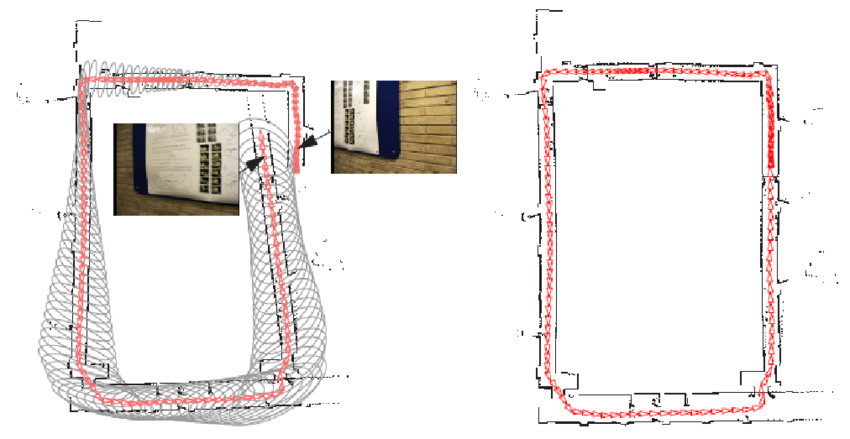
\includegraphics[width=0.7\textwidth]{loop_closure_2.png}
        \caption{Left image: Robot's path before loop closure, showing growing uncertainty (gray ellipses) and misalignment at the loop point. Camera views used for matching are inset. 
                Right image: Corrected map after loop closure, with aligned positions and reduced errors. \cite{loop_closure_2_img}}
        \label{fig:loop_closure_2}
    \end{figure}

    \newpage

    Loop closure detection faces several significant challenges:

    \textbf{Viewpoint variation}: The robot may approach the same location from a completely different direction. A corridor observed initially from north to south looks substantially different when viewed from south to north.
    
    \textbf{Perceptual aliasing}: Many environments contain similar-looking areas. In a hospital, multiple identical-looking corridors can trigger false loop closures that catastrophically distort the map.
    
    \textbf{Accumulated pose error}: By the time the robot returns to a known location, its position uncertainty may be so large that the expected and actual observations have minimal overlap.
    
    \textbf{Appearance changes}: Lighting conditions, moved objects, seasonal variations, and human activities can dramatically alter how the same location appears at different times.


    \newpage

    Modern loop closure approaches implement multi-stage processing:

    \begin{itemize}
        \item \textbf{Place recognition}: Identifying candidate locations, often using appearance-based methods such as visual bag-of-words models (DBoW), sequence-to-sequence matching, or learned embedding spaces that map 
        similar locations close together regardless of viewpoint or illumination.
        \item \textbf{Geometric verification}: Confirming candidates by establishing geometric consistency through feature matching and transformation estimation.
        \item \textbf{Global consistency checking}: Validating that the proposed loop closure is consistent with the existing map and trajectory, sometimes using techniques like RRR (Realizing, Reversing, Recovering) to reject outliers.
        \item \textbf{Graph optimization}: Incorporating verified loop closures as constraints in a pose graph that is globally optimized to distribute errors throughout the trajectory.
    \end{itemize}

    Loop closure is intimately connected with data association - the process of matching current observations with previously established map elements. While loop closure operates at the 
    level of places, data association functions across multiple levels. It enables low-level feature matching between consecutive frames for visual odometry, facilitates landmark 
    identification by associating observed features with mapped landmarks, and supports object recognition by identifying and tracking objects across multiple observations.

    While structured, static environments are reasonably well-handled by current algorithms, dynamic, changing, or visually ambiguous environments continue to pose significant difficulties that drive ongoing research.

    \section{Classical Approaches to SLAM}

    \subsection{Filter-Based Methods}
    
    Filter-based methods dominated early SLAM research, providing principled approaches to handling the inherent uncertainties in robot motion and sensing. These methods recursively estimate the posterior probability distribution over 
    robot poses and map features as new observations arrive.
    
    \textbf{Extended Kalman Filter SLAM (EKF-SLAM)} was the first widely adopted approach to SLAM. Introduced in the early 1990s, EKF-SLAM represents the joint state of the robot and map features with a multivariate Gaussian distribution, 
    maintaining both mean estimates and their uncertainty through a covariance matrix.
    
    The EKF-SLAM algorithm operates in two phases:
    \begin{itemize}
        \item \textbf{Prediction step}: Updates the state estimate based on robot motion, typically increasing uncertainty
        \item \textbf{Correction step}: Incorporates sensor measurements to update both the state estimate and reduce uncertainty
    \end{itemize}

    \begin{figure}[h!]
        \centering
        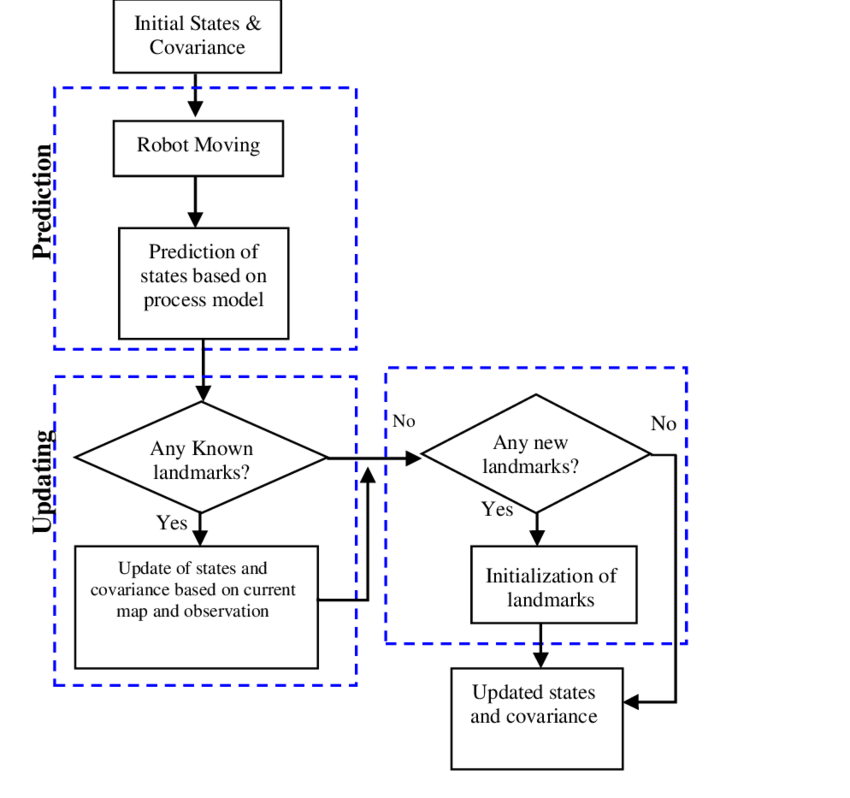
\includegraphics[width=0.7\textwidth]{D-EKF-SLAM-operation.png}
        \caption{This flowchart shows the EKF-SLAM algorithm process. Starting with initial states and covariance, it follows a prediction phase when the robot moves, 
        then branches into an update phase that either updates existing landmarks or initializes new ones, ultimately producing updated states and covariance. \cite{ekf_slam_img}}
        \label{fig:D-EKF-SLAM-operation}
    \end{figure}
    
    The mathematical formulation involves:
    \begin{itemize}
        \item State vector $\mathbf{x} = [\mathbf{x}_r, \mathbf{m}_1, \mathbf{m}_2, ..., \mathbf{m}_n]^T$ combining robot pose $\mathbf{x}_r$ and map features $\mathbf{m}_i$
        \item Covariance matrix $\mathbf{P}$ representing uncertainty in the state estimate and correlations between variables
        \item Nonlinear motion model $\mathbf{f}(\mathbf{x}, \mathbf{u})$ with control input $\mathbf{u}$
        \item Nonlinear observation model $\mathbf{h}(\mathbf{x})$ relating state to expected measurements
    \end{itemize}
    
    EKF-SLAM handles the chicken-and-egg problem by explicitly maintaining correlations between the robot pose and map features. When the robot observes a landmark, the uncertainty in both the robot's 
    position and the landmark's position becomes correlated—improving the estimate of one improves the estimate of the other.
    
    However, EKF-SLAM suffers from significant limitations:
    \begin{itemize}
        \item $O(n^2)$ computational complexity with $n$ landmarks, making it unsuitable for large-scale environments
        \item Linearization errors from the extended Kalman filter that can cause inconsistency and divergence
        \item Difficulty handling multi-modal distributions and ambiguous data associations
        \item Sensitivity to outliers in sensor measurements
    \end{itemize}
    
    \textbf{Particle Filter SLAM} addresses some EKF-SLAM limitations by representing the posterior distribution with a set of weighted samples (particles) rather than a single Gaussian. The most influential 
    particle filter approach, FastSLAM, introduced by Montemerlo et al. in 2002 \cite{fast_slam}, uses a Rao-Blackwellized particle filter that:
    \begin{itemize}
        \item Factors the SLAM posterior into robot trajectory and map features conditioned on trajectory
        \item Represents the robot trajectory distribution with particles
        \item Represents map feature estimates with compact EKFs, one per particle
    \end{itemize}
    
    This factorization leverages a key insight: conditioned on the robot trajectory, map features are independent. The FastSLAM algorithm:
    \begin{itemize}
        \item Maintains multiple trajectory hypotheses through particles
        \item Updates individual map features efficiently with separate EKFs
        \item Naturally handles multi-modal distributions and ambiguous data associations
        \item Resamples particles based on observation likelihood, removing unlikely trajectories
    \end{itemize}

    \newpage
    \begin{figure}[h!]
        \centering
        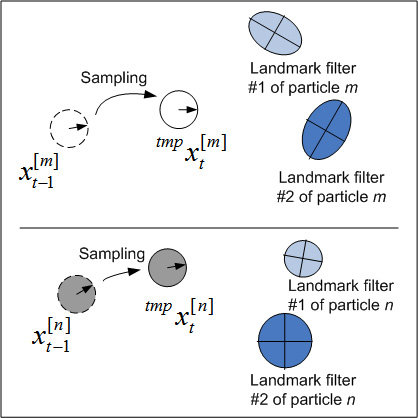
\includegraphics[width=0.7\textwidth]{fast_slam_img.png}
        \caption{This diagram shows the FastSLAM particle filter process. Two particles (m and n) are sampled from previous to temporary states. Particles represent different possible robot pose hypotheses. 
        Each particle maintains separate uncertainty estimates for two landmarks, shown as ellipses - larger ellipses indicate greater positional uncertainty. 
        Light blue ellipses represent landmark filter \#1, while darker blue ellipses represent landmark filter \#2, with the uncertainty patterns varying between particles. \cite{fast_slam_img}}
        \label{fig:fast_slam_img}
    \end{figure}
    
    FastSLAM achieves $O(M \log N)$ complexity for $M$ particles and $N$ landmarks, allowing it to scale better than EKF-SLAM to larger environments.
    
    Despite these advantages, particle filter approaches have their own limitations:
    \begin{itemize}
        \item Particle depletion in high-dimensional spaces
        \item Difficulty representing long trajectories efficiently
        \item Computational constraints on the number of particles
        \item Need for resampling, which can cause loss of diversity
    \end{itemize}
    
    Filter-based methods laid the groundwork for understanding SLAM as a probabilistic estimation problem, but their limitations in handling large-scale environments eventually 
    led to the development of more efficient optimization-based approaches.
    
    \subsection{Graph-Based Optimization}
    
    Graph-based optimization has become the dominant paradigm in modern SLAM systems, offering superior scalability and accuracy compared to filter-based methods. 
    Rather than recursively updating a state estimate, graph-based SLAM formulates the problem as finding the configuration of robot poses and map features that best explains all observations.
    
    The core idea is to represent SLAM as a sparse graph where:
    \begin{itemize}
        \item \textbf{Nodes} represent robot poses and map features
        \item \textbf{Edges} represent constraints from odometry measurements and landmark observations
    \end{itemize}
    
    This approach was pioneered by Lu and Milios in the 1990s but became practical only in the 2000s with the development of efficient optimization techniques. 
    The graph-based formulation transforms SLAM into a nonlinear least squares problem, finding the configuration of nodes that minimizes the sum of squared errors introduced by the constraints.
    
    Mathematically, we aim to find the state vector $\mathbf{x}$ that minimizes:
    
    $$\mathbf{x}^* = \arg\min_{\mathbf{x}} \sum_{i,j} \rho(\mathbf{e}_{ij}^T \mathbf{\Omega}_{ij} \mathbf{e}_{ij})$$
    
    Where:
    \begin{itemize}
        \item $\mathbf{e}_{ij}$ is the error between predicted and measured relative poses or observations
        \item $\mathbf{\Omega}_{ij}$ is the information matrix (inverse covariance) representing constraint certainty
        \item $\rho$ is a robust cost function that reduces the influence of outliers
    \end{itemize}
    
    Key advantages of graph-based SLAM include:
    \begin{itemize}
        \item \textbf{Scalability}: Sparse graph structure enables efficient optimization even for large environments
        \item \textbf{Global consistency}: Optimizes all constraints simultaneously instead of sequential filtering
        \item \textbf{Loop closure integration}: Naturally incorporates loop closures as additional constraints
        \item \textbf{Incremental operation}: Can update the solution efficiently as new information arrives
    \end{itemize}
    
    Graph-based SLAM also integrates well with both traditional and learning-based front-ends that extract constraints from sensor data. 
    The separation of front-end (data association and constraint extraction) from back-end (optimization) has enabled modular system design and focused innovation in each component.
    
    \newpage
    While graph-based optimization overcomes many limitations of filter-based methods, challenges remain:
    \begin{itemize}
        \item \textbf{Initialization sensitivity}: Performance depends on good initial values for optimization
        \item \textbf{Outlier robustness}: False constraints can significantly distort the solution
        \item \textbf{Parameter tuning}: Requires careful selection of robust cost functions and optimization parameters
    \end{itemize}
    
    Nevertheless, graph-based optimization has proven remarkably successful, becoming the foundation for most state-of-the-art SLAM systems in the last decade.
    
    \begin{figure}[h!]
        \centering
        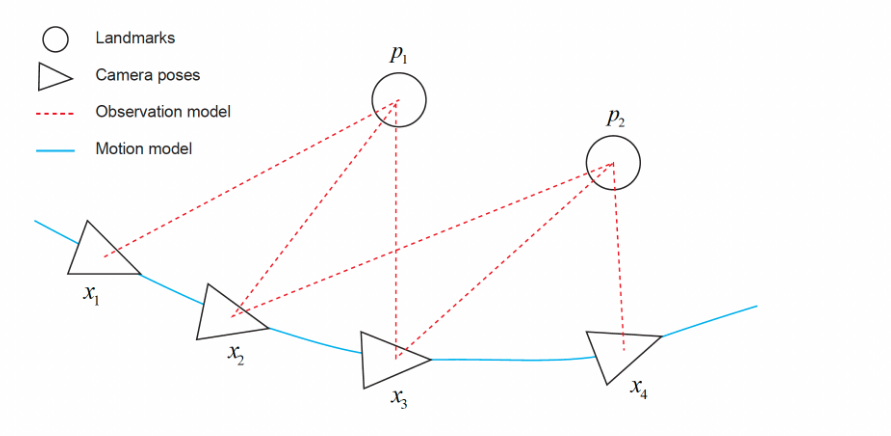
\includegraphics[width=1.1\textwidth]{graph_based_optimization.png}
        \caption{An example of the graph optimization. \cite{graph_optimization_img}}
        \label{fig:D-EKF-SLAM-operation}
    \end{figure}

    \newpage
    \subsection{Traditional Visual SLAM Systems}
    Visual SLAM systems use cameras as their primary sensing modality, offering rich environmental information at relatively low cost. Three main approaches have emerged in traditional visual SLAM:
    
    \textbf{1. Feature-based methods} detect and track distinctive points across frames, using them as landmarks. These systems typically operate through feature detection, description, matching, 
    motion estimation, and bundle adjustment to optimize camera poses and feature positions. Key innovations include parallel tracking and mapping threads and keyframe-based representations.
    
    \textbf{2. Direct methods} operate on image intensity values without extracting features, potentially using all pixels rather than sparse points. These approaches minimize photometric error rather than 
    geometric reprojection error and can work in less textured environments where feature detection might fail.
    
    \textbf{3. Hybrid approaches} combine elements of both feature-based and direct methods for increased robustness and efficiency.
    Traditional visual SLAM systems face several challenges: scale ambiguity in monocular setups, difficult initialization, sensitivity to dynamic objects and illumination changes, and poor performance in textureless regions. 
    Many systems address these limitations by incorporating additional sensing modalities like stereo cameras, RGB-D sensors, or IMUs.
    Despite impressive performance in controlled environments, traditional visual SLAM approaches still struggle with perceptual aliasing, long-term operation in changing environments, and semantic 
    understanding—limitations that have motivated the integration of learning-based methods.

    % \section{Deep Learning in Modern SLAM}
    % \subsection{Learned Features vs. Handcrafted Features}
    % \subsection{End-to-End SLAM Architectures}
    % \subsection{Neural Implicit Representations for Mapping}
    % \subsection{Depth Estimation Networks}

    % \section{Computer Vision Advancements in SLAM}
    % \subsection{Visual Odometry and Place Recognition}
    % \subsection{Semantic SLAM}
    % \subsection{Dynamic Environment Handling}

    % \section{Current Research and Applications}
    % \subsection{Self-Supervised and Few-Shot Learning}
    % \subsection{Real-World Applications}
    % \subsection{Challenges and Future Directions}

    
    \newpage
    \printbibliography[title={References}]
\end{document}